\documentclass{article}
\usepackage{amsmath}
\usepackage{graphicx}
\usepackage{tikz}
\usepackage{multicol}
\usepackage[margin=1in]{geometry}

\begin{document}
\title{Image Processing Workshop:\\ From Spatial to Frequency Domain and Back}
\author{Student Worksheet}
\date{\today}
\maketitle

\section*{Exercise 1: Understanding Basic Patterns}

\subsection*{Part A: Simple Pattern Analysis}
Consider these 5$\times$5 grayscale images. Draw their likely frequency domain representations in the empty grids.
(Key: ⚫ = strong component, ∘ = medium component, · = weak component)

\begin{center}
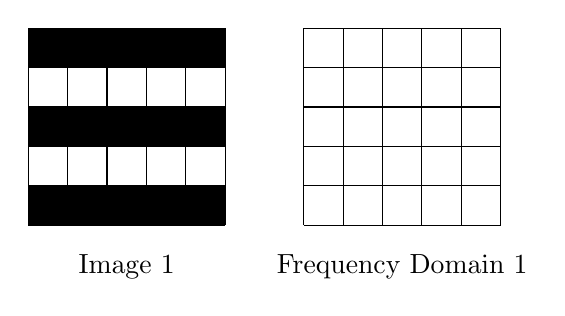
\begin{tikzpicture}[scale=0.5]
% First image - horizontal stripes
\draw (0,0) grid (5,5);
\foreach \y in {0,2,4} {
    \fill[black] (0,\y) rectangle (5,\y+1);
}
\node[below] at (2.5,-0.5) {Image 1};

% Space for frequency domain
\draw (7,0) grid (12,5);
\node[below] at (9.5,-0.5) {Frequency Domain 1};
\end{tikzpicture}
\end{center}

Your observations:
\begin{enumerate}
\item What pattern do you see in the image? \rule{8cm}{0.15mm}
\item Where would you place the main frequency components? \rule{8cm}{0.15mm}
\item Why did you place them there? \rule{8cm}{0.15mm}
\end{enumerate}

\vspace{1cm}

\section*{Exercise 2: Image Reconstruction}

\subsection*{Part A: Building from Components}
Given these frequency domain patterns, sketch the corresponding image patterns:

\begin{center}
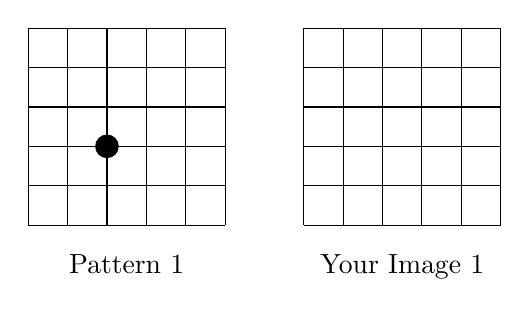
\begin{tikzpicture}[scale=0.5]
% Pattern 1 - DC only
\draw (0,0) grid (5,5);
\fill[black] (2,2) circle (0.3);
\node[below] at (2.5,-0.5) {Pattern 1};

% Space for image
\draw (7,0) grid (12,5);
\node[below] at (9.5,-0.5) {Your Image 1};
\end{tikzpicture}
\end{center}

\begin{center}
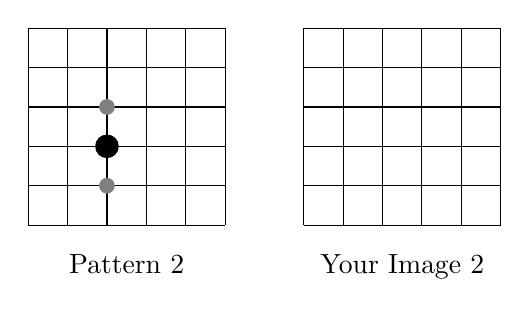
\begin{tikzpicture}[scale=0.5]
% Pattern 2 - DC + vertical component
\draw (0,0) grid (5,5);
\fill[black] (2,2) circle (0.3);
\fill[gray] (2,1) circle (0.2);
\fill[gray] (2,3) circle (0.2);
\node[below] at (2.5,-0.5) {Pattern 2};

% Space for image
\draw (7,0) grid (12,5);
\node[below] at (9.5,-0.5) {Your Image 2};
\end{tikzpicture}
\end{center}

\section*{Exercise 3: Synthesis Challenge}

Try to create an image with these characteristics:
\begin{itemize}
\item Strong vertical edge in the middle
\item Smooth gradient from left to right
\end{itemize}

\begin{enumerate}
\item First, draw your image here:
\begin{center}
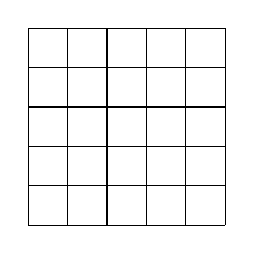
\begin{tikzpicture}[scale=0.5]
\draw (0,0) grid (5,5);
\end{tikzpicture}
\end{center}

\item Then, draw what you think its frequency components would look like:
\begin{center}
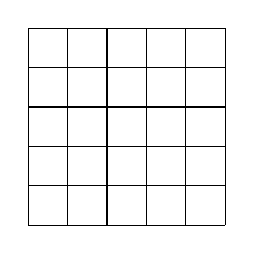
\begin{tikzpicture}[scale=0.5]
\draw (0,0) grid (5,5);
\end{tikzpicture}
\end{center}

\item Explain your reasoning: \rule{12cm}{0.15mm}
\end{enumerate}

\section*{Exercise 4: Filtering Effects}

\subsection*{Part A: Prediction}
Given this original image:
\begin{center}
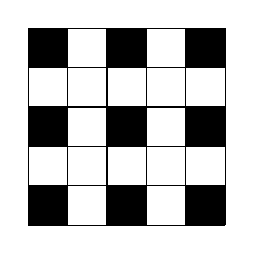
\begin{tikzpicture}[scale=0.5]
\draw (0,0) grid (5,5);
\foreach \x in {0,2,4} {
    \foreach \y in {0,2,4} {
        \fill[black] (\x,\y) rectangle (\x+1,\y+1);
    }
}
\end{tikzpicture}
\end{center}

Predict what happens when we:
\begin{enumerate}
\item Remove all high frequencies (keep only center and adjacent points)
\item Remove all horizontal frequencies
\item Keep only diagonal frequencies
\end{enumerate}

Draw your predictions:
\begin{center}
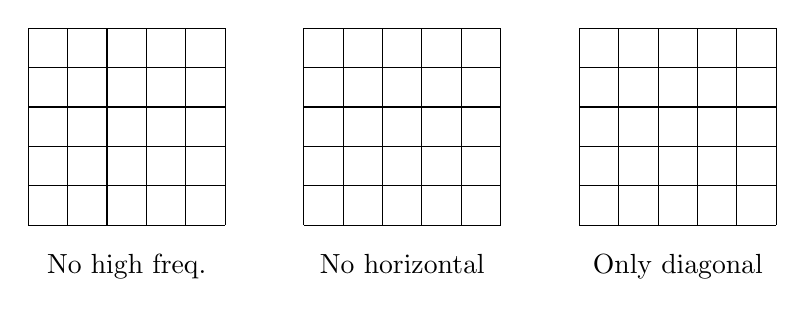
\begin{tikzpicture}[scale=0.5]
\draw (0,0) grid (5,5);
\node[below] at (2.5,-0.5) {No high freq.};

\draw (7,0) grid (12,5);
\node[below] at (9.5,-0.5) {No horizontal};

\draw (14,0) grid (19,5);
\node[below] at (16.5,-0.5) {Only diagonal};
\end{tikzpicture}
\end{center}

\section*{Exercise 5: Real World Connection}

Look at this blurry image:
\begin{center}
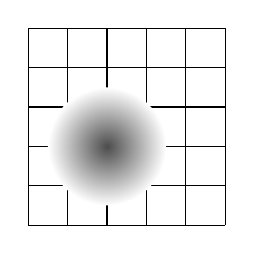
\begin{tikzpicture}[scale=0.5]
\draw (0,0) grid (5,5);
\shade[inner color=black!70,outer color=white] (2,2) circle (1.5);
\end{tikzpicture}
\end{center}

\begin{enumerate}
\item What frequencies are missing? \rule{8cm}{0.15mm}
\item How would you make it sharper? \rule{8cm}{0.15mm}
\item Draw its frequency domain representation:
\begin{center}
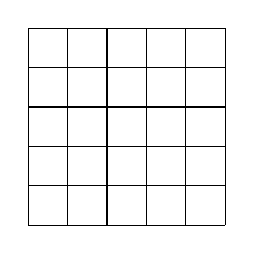
\begin{tikzpicture}[scale=0.5]
\draw (0,0) grid (5,5);
\end{tikzpicture}
\end{center}
\end{enumerate}

\vspace{1cm}
\textbf{Bonus Challenge:} Create your own pattern and its frequency representation!

\begin{center}
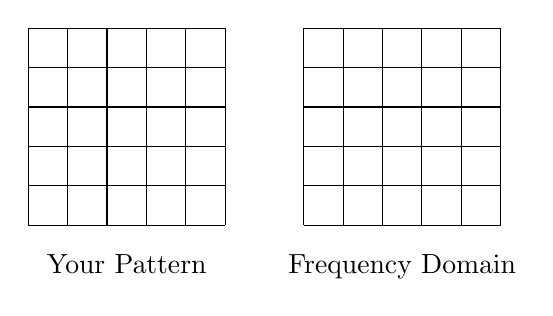
\begin{tikzpicture}[scale=0.5]
\draw (0,0) grid (5,5);
\node[below] at (2.5,-0.5) {Your Pattern};

\draw (7,0) grid (12,5);
\node[below] at (9.5,-0.5) {Frequency Domain};
\end{tikzpicture}
\end{center}

Explain why you think they match: \rule{12cm}{0.15mm}

\end{document}